\section{Quadratic Hamiltonian}

If the Hamiltonian $H$ is a sum of kinetic and potential energies, as
$H = T(p) + V(q)$, then

$$
\begin{aligned}
  (f \star_t g)(q,p) &= f\left(q_1 + t\overrightarrow{\partial_{p_1}}, \dots, p_1 - t\overrightarrow{\partial_{q_1}}, \dots\right) g(q,p) \\
  &= f(q,p) g\left(q_1 - t\overleftarrow{\partial_{p_1}}, \dots, p_1 + t\overleftarrow{\partial_{q_1}}, \dots\right) \\
  &= f\left(q_1 + t\overrightarrow{\partial_{p_1}}, \dots, p\right) g\left(q_1 - t\overleftarrow{\partial_{p_1}}, \dots, p\right)
  \end{aligned}
$$

Thus,

$$
H \star W = T(p - (i\hbar/2)\nabla_q) W + V(q +  (i\hbar/2) \nabla_p) W
$$

and similarly for the other direction. Together, it means

$$
\partial_t W = \frac{T(p - (i\hbar/2)\nabla_q) - T(p + (i\hbar/2)\nabla_q)}{i\hbar} W + \frac{V(q + (i\hbar/2)\nabla_p) - V(q - (i\hbar/2)\nabla_p)}{i\hbar} W
$$

In particular, if $T, V$ are both quadratic, such as in the case of a
harmonic oscillator $H = \frac{p^2}{2m} + \frac 12 m\omega^2 q^2$,
then we have

$$
\partial_t W = -\nabla_p T \cdot \nabla_q W + \nabla_q V \cdot \nabla_p W = \{H, W\}
$$

which is exactly the same as the classical Hamiltonian equations of
motion.

In other words, we can picture the phase-space evolution of a quantum
harmonic oscillator's Wigner function as exactly the same as if it is
the phase space evolution in classical statistical mechanics. The only
difference is that there are both regions of positive and negative
probabilities. But at least it is all real-valued!

\subsection{Free particle}

For a particle in free space, the Hamiltonian is
$H = \frac{\|p\|^2}{2m}$. Thus, the Wigner function $W$ evolves by a
simple shearing flow in phase space:

$$
W(t, q, p) = W(0, q - pt/m, p)
$$

This picture allows us to obtain some results pictorially.

\subsection{Gaussian wavepacket}

Consider the simplest case of a gaussian wavepacket on $\R$, centered
at $q = 0$, with zero total momentum. Over time, it contracts, until
its width $\sigma_q$ reaches a minimum, before spreading out again.
Let $t = 0$ be the time of minimal width, so its wavefunction
satisfies

$$
\psi(0, q) = \sqrt{\rho_{N (0, \sigma_q^2)}(q)}
$$

where $\rho_{N (0, \sigma_q^2)}$ denotes the probability density
function of the gaussian with mean $0$ and variance $\sigma_q^2$. By
direct calculation, its Wigner function is the probability density
function of the gaussian with mean $(0, 0)$ and variance
$\diag(\sigma_q^2, \sigma_p^2)$, satisfying the uncertainty principle
$\sigma_q^2 \sigma_p^2 = \hbar^2/4$.

More generally, a gaussian wavepacket with initial peak position $q_0$
and momentum $p_0$ has a Wigner function with mean $(q_0, p_0)$ and
variance $\diag(\sigma_q^2, \sigma_p^2)$. For concreteness, let
$q_0 > 0, p_0 < 0$. As time $t$ increases from $-\infty$ to
$t = 0$, the Wigner function shears to the left more and more, until
it becomes an ellipse with major axes parallel to the $p$-axis and the
$q$-axis right at $t = 0$. The center of mass on the $q$-axis is
the projection of the center of the Wigner function, which moves at
constant velocity $p_0/m$. The $q$-marginal distribution of the
Wigner function first shrinks, reaching a minimum at $t = 0$, before
growing again. Its $p$-axis marginal remains unchanged. This is shown
in the following animation.

\begin{figure}
\centering
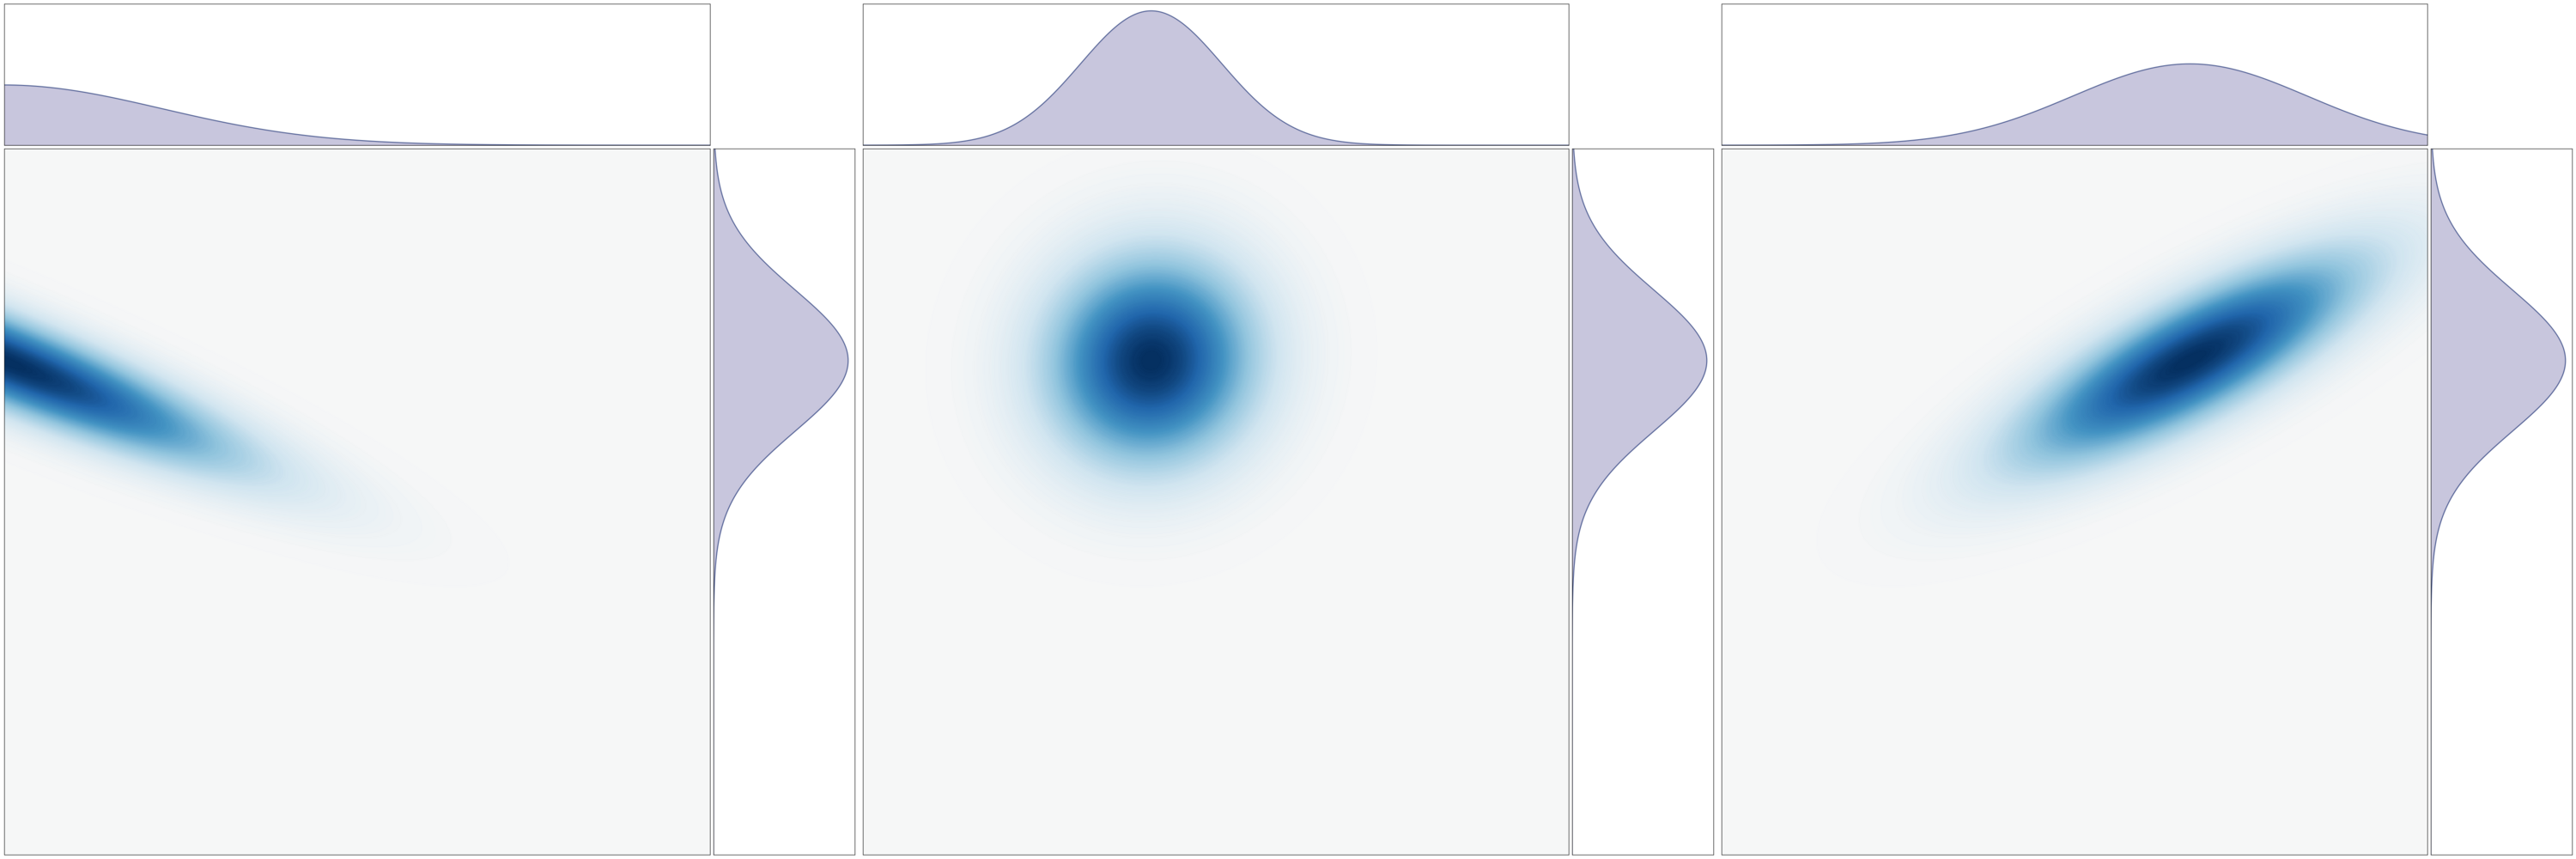
\includegraphics{figure/shear_wigner.png}
\caption{Static frames from the animation. As time increases, a gaussian
wavepacket shrinks, then spreads, on the $q$-axis marginal. Its
$p$-axis marginal remains unchanged.}
\end{figure}

\subsection{Negative probability flow}

In \cite{villanuevaNegativeFlowProbability2020; goussevCommentNegativeFlow2020}, it was noted that for a gaussian
wavepacket with positive group velocity $p_0 / m > 0$, it is often the
case that there is a paradoxical ``negative probability flow''.
Specifically, it was found that, if we stand at a point $q_1 > q_0$,
and plot $Pr(q > q_1 | t)$, the probability that the particle is found
at $q > q_1$ at time $t$, then as time passes, that probability
first decreases, before it increases, even though the wavepacket always
has positive group velocity. This is immediate in the phase space
picture.

Consider a gaussian wavepacket with
$W(0, q, p) = \rho_{N ((q_0, p_0), \diag(\sigma_q^2, \sigma_p^2))}$,
with $q_0 < 0, p_0 > 0$. Geometrically, $Pr(q > q_1 | t)$ is the
integral of $W(t, q, p)$ on the region to the right of the vertical
line $q = q_1$, which is equal to the integral of $W(0, q, p)$ on
the region to the right of the sheared line $q = -\frac{t}{m} p$. The
sheared line rotates clockwise over time.

From the geometry of gaussian distributions, this integral can be
pictorially calculated by finding the ellipse of constant
$\rho_{N ((q_0, p_0), \diag(\sigma_q^2, \sigma_p^2))}$ that is tangent
to the sheared line. At $t \to -\infty$, the sheared line is just the
$q$-axis. As $t$ increases, the sheared line rotates
counterclockwise, and the tangent ellipse grows, until it hits the
maximal size at some critical time $t = t_{\text{critical}}$, at which
point the tangent ellipse is equal to

$$
\frac{(q-q_0)^2}{\sigma_q^2} + \frac{(p-p_0)^2}{\sigma_p^2} = \frac{(q_1-q_0)^2}{\sigma_q^2} + \frac{(0-p_0)^2}{\sigma_p^2}
$$

It is a simple exercise to show
$t_{\text{critical}} = -\frac{mp_0 \sigma_q^2}{(q_1- q_0) \sigma_p^2}$.

After that, the tangent ellipse shrinks again. This is illustrated in
the following figure.

\begin{figure}
\centering
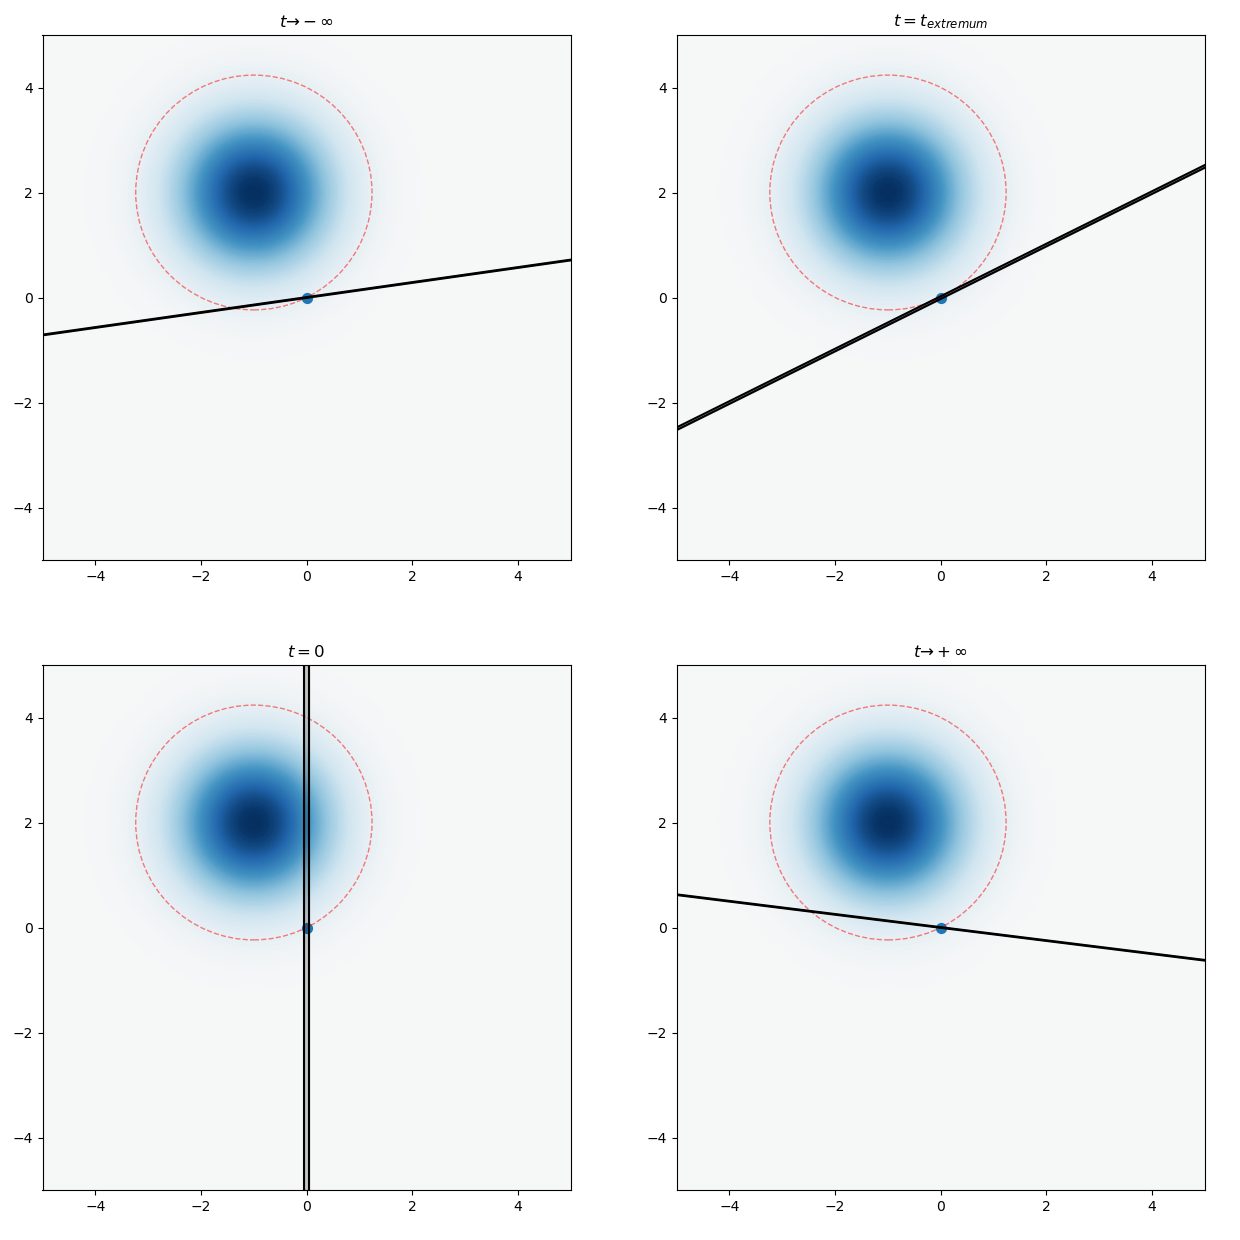
\includegraphics{figure/negative_probability_flow.png}
\caption{Illustration for the negative probability flow of a gaussian
wavepacket. The dashed circle is the largest possible tangent ellipse.
At $t = t_{\text{critical}}$, the sheared line is tangent to the
dashed circle.}
\end{figure}

By tracing out the pictures, we visually see that $Pr(q > q_1|t)$
decreases over the region $t \leq t_{\text{critical}}$, and increases
over the region $t \geq t_{\text{critical}}$.

By a similar pictorial reasoning, if $q_0 > 0, p_0 > 0$, then
$Pr(q > q_1|t)$ increases over the region
$t \leq t_{\text{critical}}$, and decreases over the region
$t \geq t_{\text{critical}}$. Only when $q_0 = q_1$ is
$Pr(q > q_1|t)$ strictly monotonic over all time.

\subsection{Wave dispersion}

As noted previously, a gaussian wave packet first shrinks, then grows,
according to a precise formula proved in every introductory quantum
mechanics course. We derive this formula geometrically.

Without loss of generality, consider a wavepacket with zero group
velocity, centered at $q = 0$, reaching minimal width $\sigma_q$ at
$t=0$. Its Wigner function is
$\rho_{N((0, 0), \diag(\sigma_q^2, \sigma_p^2))}$, where
$\sigma_q \sigma_p = \hbar / 2$.

Now, consider its one-sigma ellipse
$\frac{q^2}{\sigma_q^2} + \frac{p^2}{\sigma_q^2} = 1$. It projects to
an interval $[-\sigma_q, +\sigma_q]$ on the $q$-axis, meaning that
at time $t=0$, the probability of finding the particle within the
interval $[-\sigma_q, +\sigma_q]$ is plus-or-minus one-sigma, that is,
68.3\%.

Now, at time $t$, the new one-sigma interval can be either found by
shearing the Wigner function, or by shearing the $q$-intervals. As
pictured, the sheared $q$-intervals are the tangent lines to the
one-sigma ellipse satisfying $q + \frac{t}{m} p = C$. The tangent
points are

$$
(q, p) = \left( \frac{\sigma_q}{\sqrt{1 + \left( \frac{\sigma_p t}{\sigma_q m}\right)^2}}, \frac{\sigma_p}{\sqrt{1 + \left( \frac{\sigma_p t}{\sigma_q m}\right)^{-2}}}\right)
$$

and so, the projection to the $q$-axis has end points

$$
\pm \sigma_q\sqrt{1 + \left( \frac{\sigma_p t}{\sigma_q m}\right)^2} = \pm \sqrt{\sigma_q^2 + \left( \frac{\hbar t}{2m\sigma_q}\right)^2}
$$

as expected.

\begin{figure}
\centering
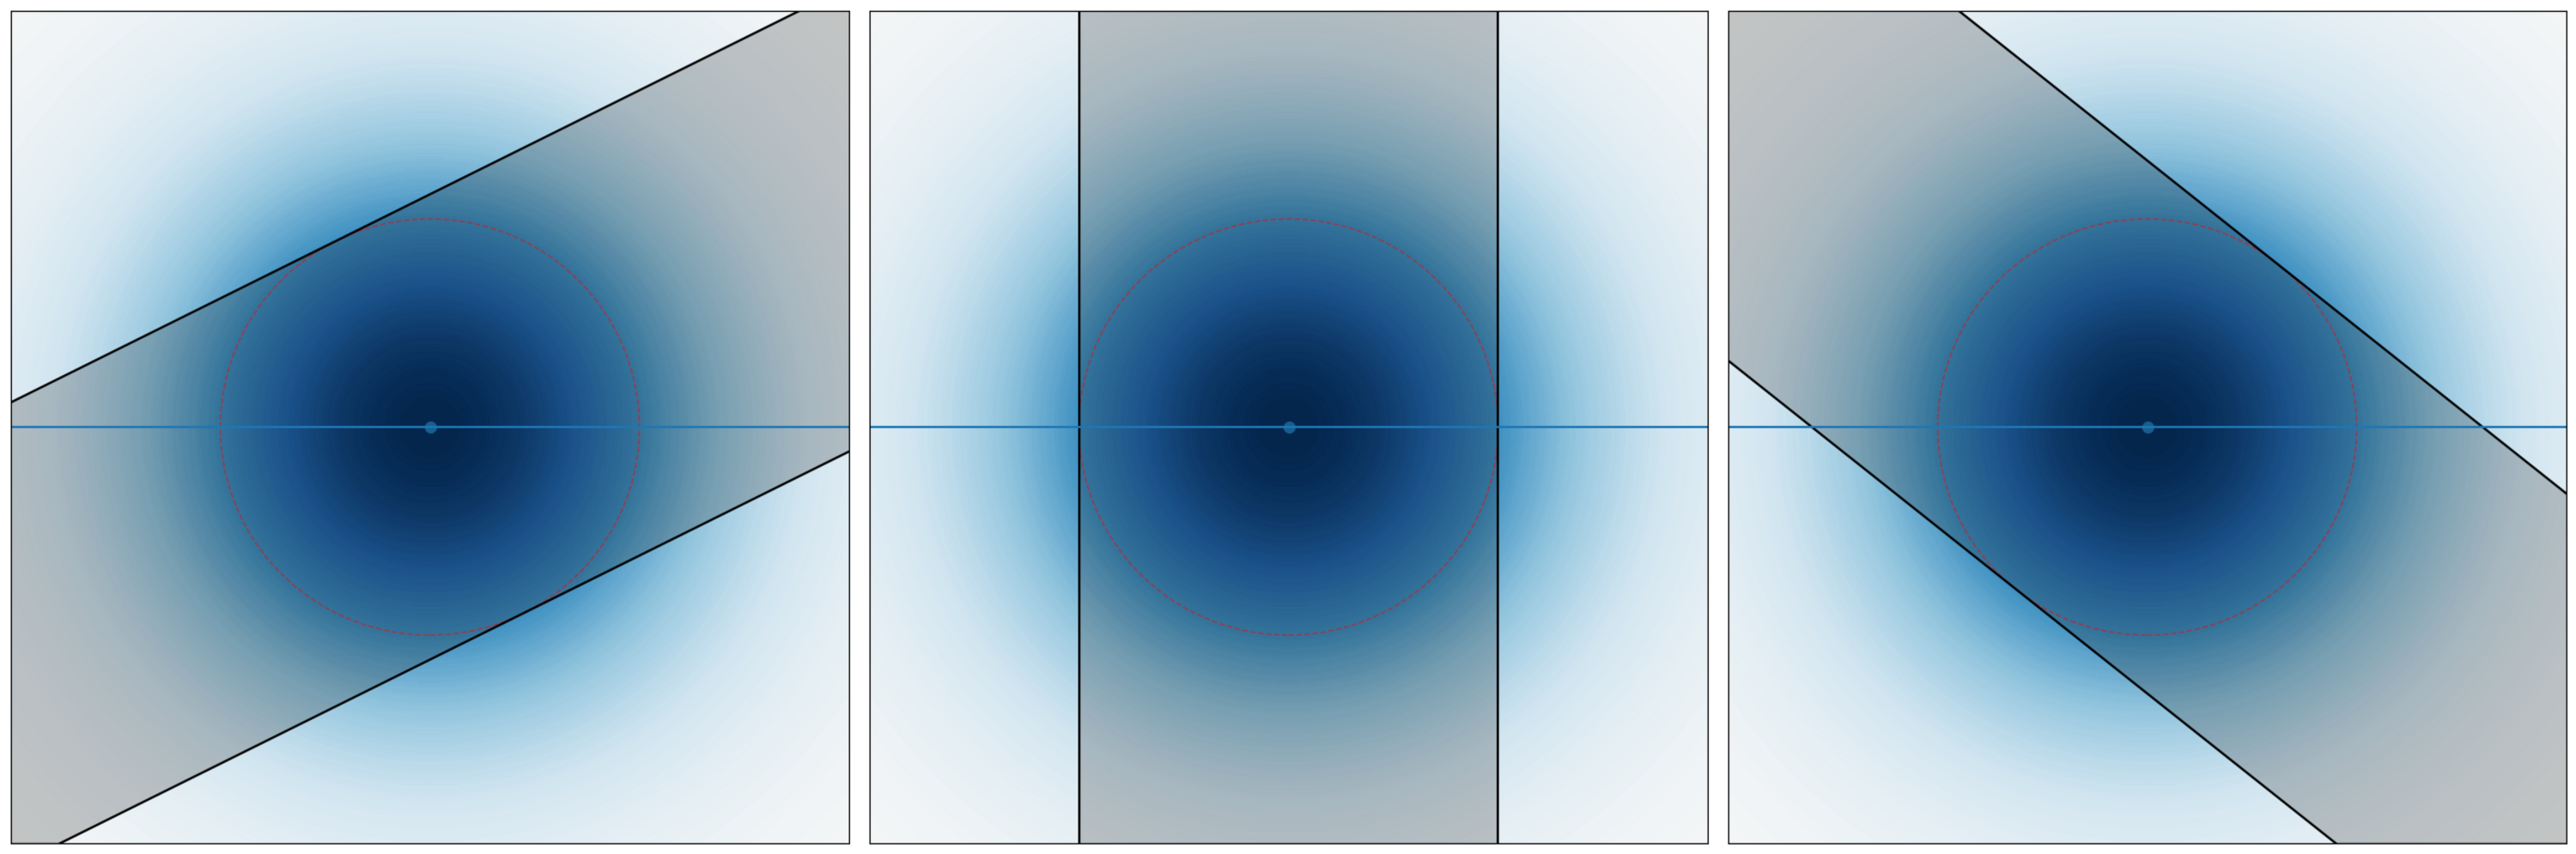
\includegraphics{figure/gaussian_wavepacket_spreading.png}
\caption{Illustration for gaussian wavepacket spreading. As time
increases, the one-sigma circle projects to an interval on $q$-axis,
which shrinks as $t \uparrow 0$, then grows as $t \uparrow \infty$.}
\end{figure}

In particular, for very large $t$, the wavepacket spreads linearly.
This is in fact a generic result for arbitrary waves. Specifically, the
$q$-marginal of the Wigner function at $q = q_1$ and time $t$ can
be found by shearing a thin slice $q \in [q_1, q_1 + \delta q]$ back
by $\frac{pt}{m}$. If $t$ is large, then this thin slice,
perpendicular to the $q$-axis, is sheared to become almost
perpendicular to the $p$-axis instead, which is approximately
$p \in [mq_1 / t, m(q_1 + \delta q)/ t]$. Thus, we have

$$
|\psi_q(t, q)|^2 \to \frac{m}{t}|\psi_p(0, mq_1 / t)|^2
$$

as $t \to +\infty$.

\subsection{Hermite--Gauss waves}

For a simple harmonic oscillator with Hamiltonian
$\frac{p^2}{2m} + \frac 12 m\omega^2 q^2$, the evolution of the Wigner
function is still the same as the classical one. Thus, the Wigner
function simply rotates in phase space. A standing wave for a simple
harmonic oscillator, then, is some wavefunction $\psi(q)$ such that
its Wigner function is rotationally symmetric.

It is proved in every introductory quantum mechanics course that such
standing waves are precisely the Hermite--Gauss waves:

$$
\psi_n(x) = \frac{1}{\sqrt{2^n\,n!}}  \left(\frac{m\omega}{\pi \hbar}\right)^{1/4}  e^{
- \frac{m\omega x^2}{2 \hbar}} H_n\left(\sqrt{\frac{m\omega}{\hbar}} x \right), \qquad n = 0,1,2,\ldots.
$$

where $H_n$ are the
\href{https://en.wikipedia.org/wiki/Hermite_polynomials}{physicist's
Hermite polynomials}. Therefore, by the previous picture of how the
probability density spreads, we conclude that

\leavevmode\vadjust pre{The Hermite--Gauss waves are the only wavefunctions whose probability
density functions retain their shapes during propagation in free space.

Furthermore, the exact same argument as the previous section allows us
to compute how fast the wave spreads. Though the $q$-marginal is no
longer gaussian, we can still characterize its width by a single number.

Concretely, let $t=0$ be the point in time where the wave has minimal
spread -- that is, the point at which its Wigner function has contour
ellipses that are not tilted, but has major axes parallel to the
$q$-axis and the $p$-axis. Let $\sigma_q$ be the quartile
distance. That is, between $q_{50\%}$ and $q_{75\%}$, where
$q_{75\%}$ is the point such that $Pr(q \leq q_{75\%}) = 75\%$.

Since in the simple harmonic oscillator, the Wigner function just
rotates around classically, we can calculate as if it is classical. This
means that the energy conservation holds:

$$
\frac{\sigma_p(0)^2}{2m} = \frac 12 m\omega^2 \sigma_q(0)^2 \implies \sigma_p(0)/\sigma_q(0) = m\omega
$$

Now, the same geometric argument shows that

$$
\sigma_q(t) = \sigma_q(0)\sqrt{1 + \left( \frac{\sigma_p(0) t}{\sigma_q(0) m}\right)^2} = \sigma_q(0)\sqrt{1 + \left(\omega t\right)^2}
$$

which is a surprisingly simple and elegant formula. The case of the
gaussian is recovered by noting that it is the only Hermite--Gauss wave
that exactly reaches the minimum allowed by the uncertainty principle:
$\sigma_q(0) \sigma_p(0) = \hbar/2$, which, when combined with
$\sigma_p(0)/\sigma_q(0) = m\omega$ that is satisfied by all
Hermite--Gauss waves, gives us
$\omega = \frac{\hbar}{2 m \sigma_q^2}$, and so we recover the
previous result of
$\sigma_q(t) = \sigma_q(0)\sqrt{1 + \left(\frac{\hbar t}{2 m \sigma_q^2}\right)^2}$

\begin{figure}
\centering
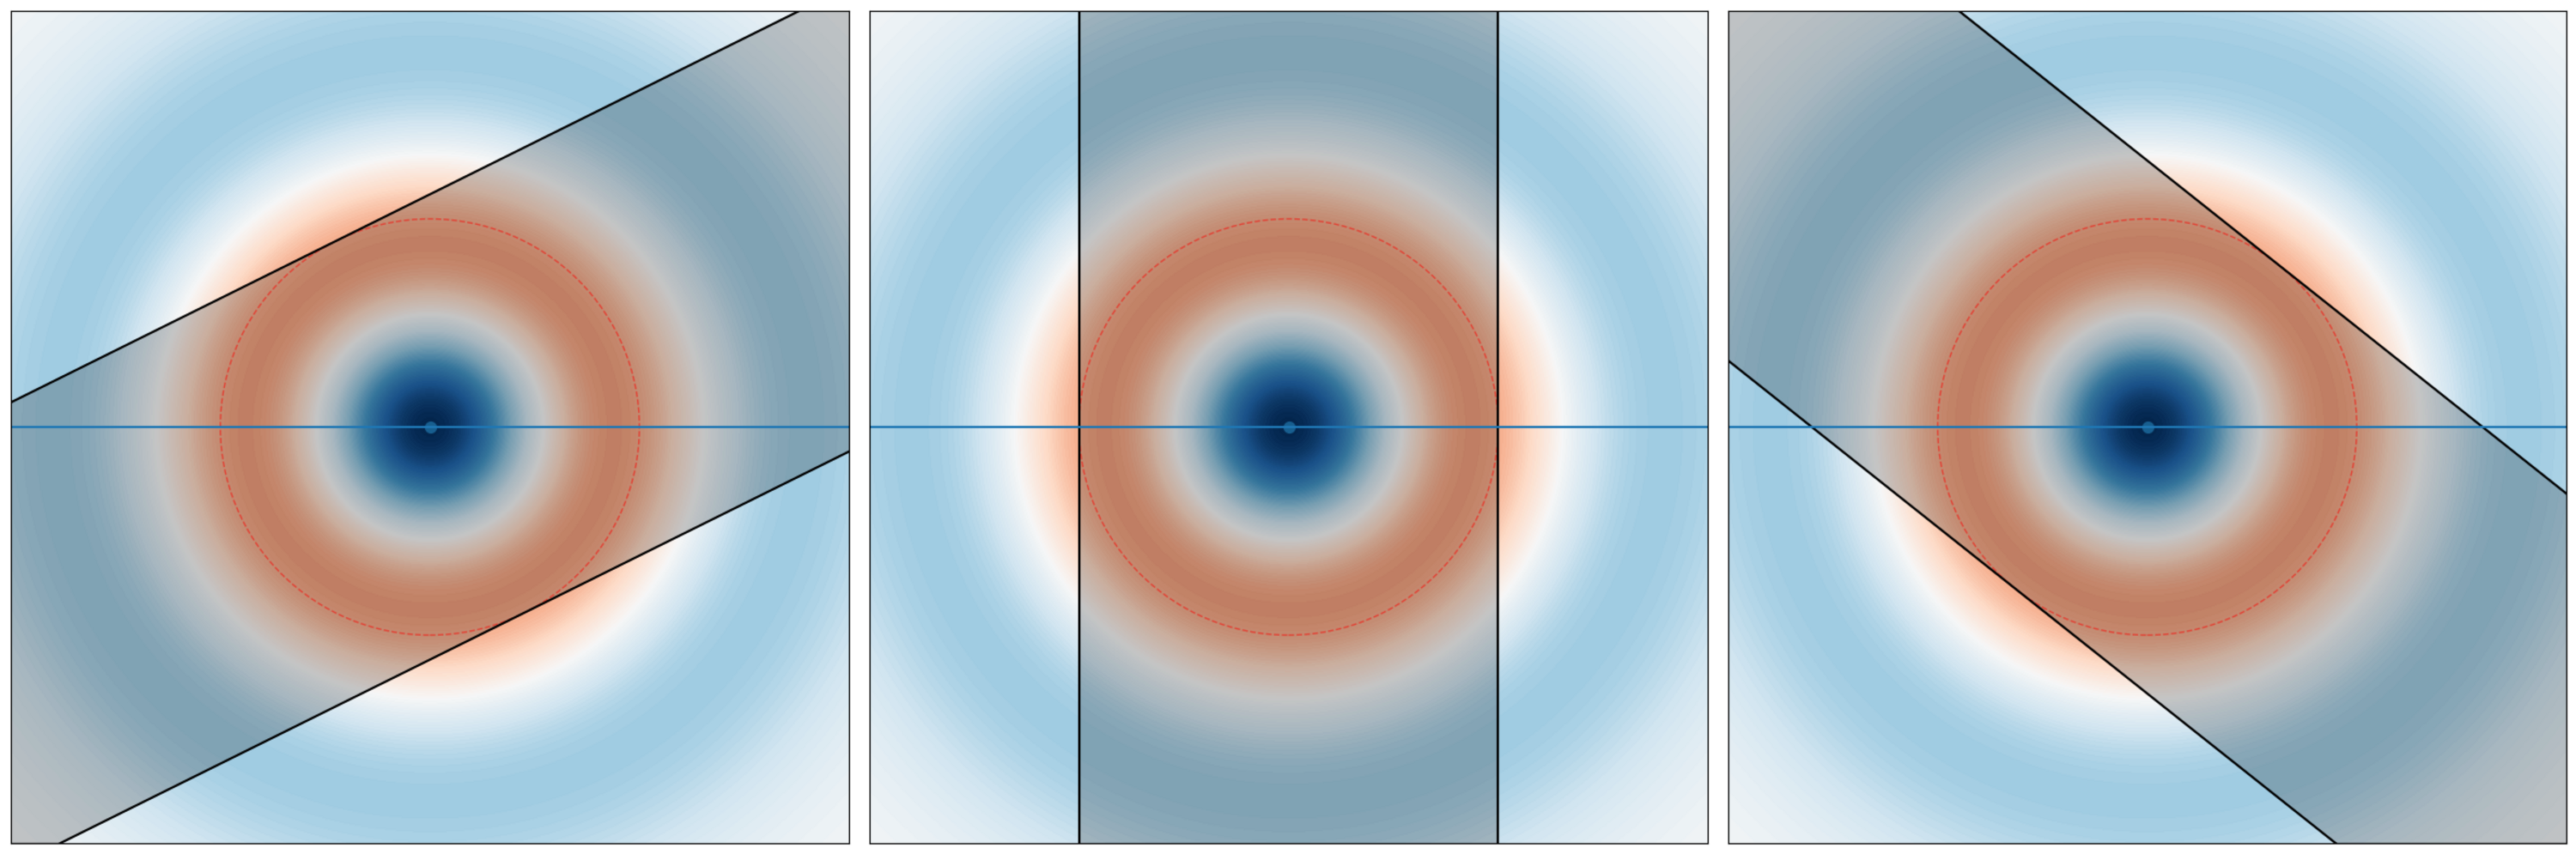
\includegraphics{figure/gaussian_wavepacket_spreading_2.png}
\caption{Illustration for gaussian wavepacket spreading in a
wavefunction corresponding to the $n=2$ eigenstate of the simple
harmonic oscillator. As time increases, the one-sigma circle projects to
an interval on $q$-axis, which shrinks as $t \uparrow 0$, then grows
as $t \uparrow \infty$.}
\end{figure}

These results were previously proved in
\cite{andrewsEvolutionFreeWave2008} analytically. However as far as the
author knows, this is the first time these were derived geometrically,
with minimal calculus.

\subsection{Square wave}

As a concrete example of a wave that is not Hermite--Gauss, consider the
square wave function

$$
\psi(q) = \begin{cases}a^{-1/2} & \text{ if }q \in [-a/2, +a/2]\\ 0  & \text{ else}\end{cases}
$$

Its Wigner function is easily calculated as

$$
\begin{aligned}
      W_0(q, p) &= \frac{1}{2a\pi \hbar} \int_{|q + y/2| \leq a/2, |q - y/2| \leq a/2} dy e^{-ipy /\hbar} \\
      &= \frac{1}{2a\pi \hbar} \frac{\hbar}{-ip} e^{-ipy /\hbar}\Big|_{\max(2q - a, -2q- a)}^{\min(2q+a, -2q+a)}\\
      &= \frac{1}{a \pi p} \sin\left(\frac{p(a - 2|q|)}{\hbar} \right)
      \end{aligned}
$$

when $q \in [-a/2, +a/2]$. For larger values, $W = 0$.

The $p$-marginal distribution is

$$
\begin{aligned}
\rho_p(p) &:= \int_\R  W_0(q,p)dq  \\
      &= \int_{-a/2}^{+a/2} \frac{1}{a \pi p} \sin\left(\frac{p(a - 2|q|)}{\hbar} \right) dq \\
      &= \frac{\hbar }{\pi a p^2} ( 1 - \cos(pa /\hbar))
\end{aligned}
$$

Let
$f(t) := \frac{1 - \cos t}{\pi t^2} = \left(\frac{\operatorname{sinc}(t/2)}{\sqrt{2\pi}} \right)^2$,
then $\rho_p(p) = \frac{a}{\hbar} f(\frac{a}{\hbar}p)$. Thus, the
$p$-marginal distribution always has the same shape no matter what
$a$ is.

\begin{figure}
\centering
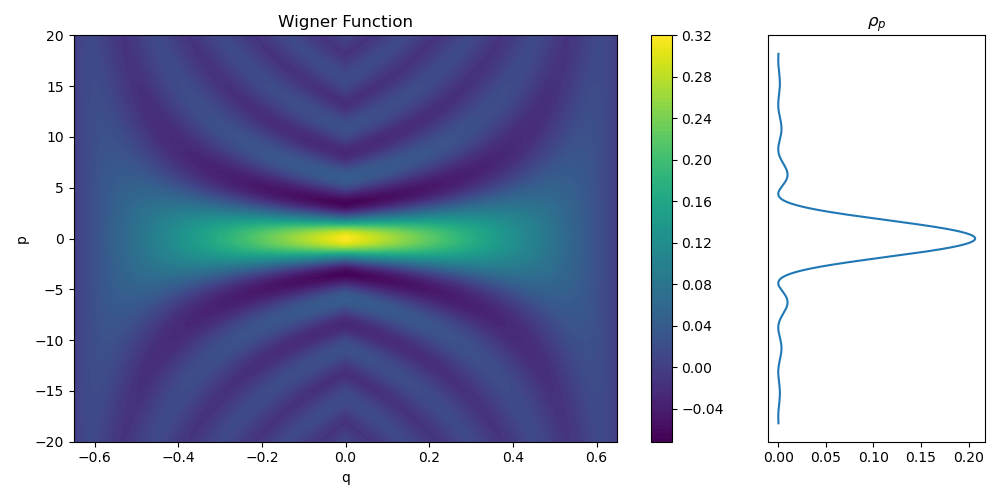
\includegraphics{figure/square_wave_wigner.png}
\caption{Wigner function of the square wave, and its $p$-marginal
distribution. $a = 1.3, \hbar = 1$}
\end{figure}

Because at $t=0$, the Wigner function is zero outside of
$q \in [-a/2, +a/2]$, at large $t$, the probability that the
particle is found at $[q, q + \delta q]$ is the integral of $W_0$
over a the thin line passing $[q, q + \delta q]$ at slope $-m/t$.
Thus, we have

$$
\begin{aligned}
\int_\R W_t(q, p)dp 
    &\approx \frac mt\int_{-a/2}^{+a/2} W_0(q, p)dq \\
    &= \frac{m}{t} \rho_p(qm/t) = \frac{\hbar t}{\pi m a q^2} \left(1 - \cos \left( \frac{ma}{\hbar t} q\right)\right) \\
    &= \frac{am}{\hbar t} f \left(\frac{am}{\hbar t} q\right)
\end{aligned}
$$

In particular, the higher-order waves are \emph{not} disspated away, and
so the square wave never converges to a gaussian wavepacket. In fact, it
always converges to the same shape of $f$. This is directly against
the claim of \cite{mitaDispersionNonGaussianFree2007}, as previously
pointed out by \cite{andrewsEvolutionFreeWave2008}.

By the symmetry of the Wigner function in $q$ and $p$, we have the
following result: If the wavefunction satisfies
$\psi(q) = \sqrt{\frac{b}{\hbar} }\frac{\operatorname{sinc}(bq/2 \hbar)}{\sqrt{2\pi}}$
at $t=0$, then at large $t$, the wavefunction converges to a square
wave on the interval $[-bt/2m, +bt/2m]$ with height
$\sqrt{\frac{m}{bt}}$.

\subsection{Generic wavepacket}

In general, the shape of the wave of any normalizable wave function
$\psi_q(q)$, propagating in free space, would, after a long time,
converge to a translation-and-dilation of its $p$-marginal
distribution $\psi_q(q)$, multiplied by a phase factor
$e^{iS(t, q)}$. Since the $q$-marginal distribution can be
arbitrary, the same is true for the $p$-marginal distribution. In
particular, we have the following theorem, which is immediate from the
geometric intuition.

\leavevmode\vadjust pre{If $\rho$ is a smooth probability density function on $\R$, then
there exists a wavefunction $\psi$ propagating in free space, such
that for all large enough $t$,

$$
|\psi(t, q)|^2 \to \frac{m}{t}\rho(mq/t)
$$

Such $\psi(0, q)$ can be found by taking the Wigner function of
$\sqrt{\rho(p)} e^{iS(p)}$ for an arbitrary smooth function $S$,
rotating by 90 degrees in the phase plane, then taking the inverse
Wigner transform.

Previously, we showed that for almost any gaussian wavepacket,
$Pr(q > q_1 | t)$ the probability of finding the particle to the right
of some point $q_1$ at time $t$, would first increase then decrease,
or first decrease then increase. In fact, this is true for almost any
Wigner function, period. The Wigner function does not even need to be
pure. It can be the Wigner function of a mixed state, and this would
still be true.

\leavevmode\vadjust pre{For almost any mixed state of a particle propagating in free space, and
almost any $q_1$, the function $t \mapsto Pr(q > q_1 | t)$ is not
monotonic.

Fix some Wigner function $W$. Define $f(\theta)$ to be the integral
of $W$ to the right of the line passing $(q_1, 0)$, making an angle
$\theta$ with the $q$-axis. Then we have $f(0) = 1 - f(\pi)$, and
in general, $f(\theta) = 1 - f(\pi + \theta)$. Thus, if $f$ reaches
a global minimum at $\theta$, then it reaches a global maximum at
$f(\theta + \pi)$. In particular, if $f(0)$ is neither the global
minimum nor the global maximum, then $f(\theta)$ must reach either the
global minimum or the global maximum at some $\theta \in (0, \pi)$.
Therefore, $f$ is not monotonic as $\theta$ rotates.

We can think of this as a ``maximally non-dissipation'' result. Unlike
the heat equation, where all high-frequency fluctuations decay away,
leaving behind just a single low-frequency gaussian mode, the
Schrödinger equation results in a wave propagation that has no
dissipation, but preserves the shape of $|\psi_p(0)|^2$ for all large
times. This is unsurprising, as it is well-known that quantum mechanics
does not dissipate.
